
The CMake Language wouldn't be complete without control structures! Like everything else, they are provided in the form of a command, and they come in three categories: conditional blocks, loops, and command definitions. Control structures are executed in scripts and during buildsystem generation for projects.

\subsubsubsection{2.5.1\hspace{0.2cm}Conditional blocks}

The only conditional block supported in CMake is the humble if() command. All conditional blocks have to be closed with an endif() command, and they may have any number of elseif() commands and one optional else() command in this order:

\begin{lstlisting}[style=styleCMake]
if(<condition>)
	<commands>
elseif(<condition>) # optional block, can be repeated
	<commands>
else() # optional block
	<commands>
endif()
\end{lstlisting}

As in many other imperative languages, the if()-endif() block controls which sets of commands will be executed:

\begin{itemize}
\item 
If the <condition> expression specified in the if() command is met, the first section will be executed.

\item 
Otherwise, CMake will execute commands in the section belonging to the first elseif() command in this block that has met its condition.

\item 
If there are no such commands, CMake will check if the else() command is provided and execute any commands in that section of the code.

\item 
If none of the above conditions are met, the execution continues after the endif() command.
\end{itemize}

The provided <condition> expression is evaluated according to a very simple syntax.

\subsubsubsection{2.5.2\hspace{0.2cm}The syntax for conditional commands}

The same syntax is valid for if(), elseif(), and while() commands.

\hspace*{\fill} \\ %插入空行
\noindent
\textbf{Logical operators}

The if() conditions support the NOT, AND, and OR logical operators:

\begin{itemize}
\item 
NOT <condition>

\item 
<condition> AND <condition>

\item 
<condition> OR <condition>
\end{itemize}

Also, the nesting of conditions is possible with matching pairs of parentheses (()). As in all decent languages, the CMake Language respects the order of evaluation and starts from the innermost parenthesis:

\begin{itemize}
\item 
(<condition>) AND (<condition> OR (<condition>))
\end{itemize}

\hspace*{\fill} \\ %插入空行
\noindent
\textbf{The evaluation of a string and a variable}

For legacy reasons (because the variable reference (\$\{\}) syntax wasn't always around), CMake will try to evaluate unquoted arguments as if they are variable references. In other words, using a plain variable name (for example, VAR) inside a condition is equal to writing \$\{VAR\}. Here's an example for you to consider, and a gotcha:

\begin{lstlisting}[style=styleCMake]
set(VAR1 FALSE)
set(VAR2 "VAR1")
if(${VAR2})
\end{lstlisting}

The if() condition works in a bit of a convoluted way here – first, it will evaluate \$\{VAR2\} to VAR1, which is a recognized variable, and this in turn is evaluated to the FALSE string. Strings are considered Boolean true only if they equal any of the following constants (these comparisons are case insensitive):

\begin{itemize}
\item 
ON, Y, YES, or TRUE

\item 
A non-zero number
\end{itemize}

This brings us to the conclusion that the condition in the preceding example will evaluate to false.

However, here's another catch – what would be the evaluation of a condition with an unquoted argument with a name of a variable containing a value such as BAR? Consider the following code example:

\begin{lstlisting}[style=styleCMake]
set(FOO BAR)
if(FOO)
\end{lstlisting}

According to what we have said so far, it would be false, as the BAR string doesn't meet the criteria to evaluate to a Boolean true value. That's unfortunately not the case, because CMake makes an exception when it comes to unquoted variable references. Unlike with quoted arguments, FOO won't be evaluated to BAR to produce an if("BAR") statement (which would be false). Instead, CMake will only evaluate if(FOO) to false if it is any of the following constants (these comparisons are case insensitive):

\begin{itemize}
\item 
OFF, NO, FALSE, N, IGNORE, NOTFOUND

\item 
A string ending with -NOTFOUND

\item 
An empty string

\item 
Zero
\end{itemize}

So, simply asking for an undefined variable will be evaluated to false:

\begin{lstlisting}[style=styleCMake]
if (FOO)
\end{lstlisting}

However, defining a variable beforehand changes the situation, and the condition is evaluated to true:

\begin{lstlisting}[style=styleCMake]
set(FOO "FOO")
if (FOO)
\end{lstlisting}

\begin{tcolorbox}[colback=blue!5!white,colframe=blue!75!black,title=Note]
If you think that the behavior of unquoted arguments is confusing, wrap variable references in quoted arguments: if ("\$\{FOO\}"). This will result in argument evaluation before the provided argument is passed into the if() command, and the behavior will be consistent with the evaluation of strings.
\end{tcolorbox}

In other words, CMake assumes that the user is asking if the variable is defined (and is not explicitly false). Luckily, we can explicitly check that fact (and not worry about the value inside):

\begin{lstlisting}[style=styleCMake]
if(DEFINED <name>)
if(DEFINED CACHE{<name>})
if(DEFINED ENV{<name>})
\end{lstlisting}

\hspace*{\fill} \\ %插入空行
\noindent
\textbf{Comparing values}

Comparison operations are supported with the following operators:

EQUAL, LESS, LESS\_EQUAL, GREATER, and GREATER\_EQUAL

They can be used to compare numeric values, like so:

\begin{lstlisting}[style=styleCMake]
if (1 LESS 2)
\end{lstlisting}

\begin{tcolorbox}[colback=blue!5!white,colframe=blue!75!black,title=Note]
The CMake documentation states that if one of the operands is not a number, the value will be false. But practical experiments show that the comparison of strings starting with a number works correctly: if (20 EQUALS "20 GB").
\end{tcolorbox}

You can compare software versions following the major[.minor[.patch[.tweak]]] format by adding a VERSION\_ prefix to any of the operators:

\begin{lstlisting}[style=styleCMake]
if (1.3.4 VERSION_LESS_EQUAL 1.4)
\end{lstlisting}

Omitted components are treated as zero, and non-integer version components truncate the compared string at that point.

For lexicographic string comparisons, we need to prepend an operator with the STR prefix (note the lack of an underscore):

\begin{lstlisting}[style=styleCMake]
if ("A" STREQUAL "${B}")
\end{lstlisting}

We often need more advanced mechanisms than simple equality comparisons.

Fortunately, CMake also supports POSIX regex matching (the CMake documentation hints at an ERE flavor, but no support for specific regex character classes is mentioned).

We can use the MATCHES operator as follows: <VARIABLE|STRING> MATCHES <regex> Any matched groups are captured in CMAKE\_MATCH\_<n> variables.

\hspace*{\fill} \\ %插入空行
\noindent
\textbf{Simple checks}

We already mentioned one simple check, DEFINED, but there are others that simply return true if a condition is met.

We can check the following:

\begin{itemize}
\item 
If a value is in a list: <VARIABLE|STRING> IN\_LIST <VARIABLE>

\item 
If a command is available for invocation: COMMAND <command-name>

\item 
If a CMake policy exists: POLICY <policy-id> (this is covered in Chapter 3, Setting Up Your First CMake Project)

\item 
If a CTest test was added with add\_test(): TEST <test-name>

\item 
If a build target is defined: TARGET <target-name>
\end{itemize}

We'll explore build targets in Chapter 4, Working with Targets, but for now, let's just say that targets are logical units of a build process in a project created with a add\_executable(), add\_library(), or add\_custom\_target() command that has already been invoked.

\hspace*{\fill} \\ %插入空行
\noindent
\textbf{Examining the filesystem}

CMake provides many ways of working with files. We rarely need to manipulate them directly, and normally we'd rather use a high-level approach. For reference, this book will provide a short list of the file-related commands in the Appendix section. But most often, only the following operators will be needed (behavior is well defined only for absolute paths):

\begin{itemize}
\item 
EXISTS <path-to-file-or-directory>: Checks if a file or directory exists 

This resolves symbolic links (it returns true if the target of the symbolic link exists).

\item 
<file1> IS\_NEWER\_THAN <file2>: Checks which file is newer

This returns true if file1 is newer than (or equal to) file2 or if one of the two files doesn't exist.

\item 
IS\_DIRECTORY path-to-directory: Checks if a path is a directory

\item 
IS\_SYMLINK file-name: Checks if a path is a symbolic link

\item 
IS\_ABSOLUTE path: Checks if a path is absolute
\end{itemize}

\subsubsubsection{2.5.3\hspace{0.2cm}Loops}

Loops in CMake are fairly straightforward – we can use either while() or foreach() to repeatedly execute the same set of commands. Both of these commands support loop control mechanisms:

\begin{itemize}
\item 
The break() loop stops the execution of the remaining block and breaks from the enclosing loop.

\item 
The continue() loop stops the execution of the current iteration and starts at the top of the next one.
\end{itemize}

\hspace*{\fill} \\ %插入空行
\noindent
\textbf{While}

The loop block is opened with a while() command and closed with an endwhile() command. Any enclosed commands will be executed as long as the <condition> expression provided in while() is true. The syntax for phrasing the condition is the same as for the if() command:

\begin{lstlisting}[style=styleCMake]
while(<condition>)
	<commands>
endwhile()
\end{lstlisting}

You probably guessed that – with some additional variables – the while loop can replace a for loop. Actually, it's way easier to use a foreach() loop for that – let's take a look.

\hspace*{\fill} \\ %插入空行
\noindent
\textbf{Foreach loops}

A foreach block comes in a few variants that execute enclosed commands for each value. Like other blocks, it has opening and closing commands: foreach() and endforeach().

The simplest form of foreach() is meant to provide a C++-style for loop:

\begin{lstlisting}[style=styleCMake]
foreach(<loop_var> RANGE <max>)
	<commands>
endforeach()
\end{lstlisting}

CMake will iterate from 0 to <max> (inclusive). If we need more control, we can use the second variant, providing <min>, <max>, and, optionally, <step>. All arguments must be nonnegative integers. Also, <min> has to be smaller than <max>:

\begin{lstlisting}[style=styleCMake]
foreach(<loop_var> RANGE <min> <max> [<step>])
\end{lstlisting}

However, foreach() shows its true colors when it is working with lists:

\begin{lstlisting}[style=styleCMake]
foreach(<loop_variable> IN [LISTS <lists>] [ITEMS <items>])
\end{lstlisting}

CMake will take elements from all of the provided <lists> list variables, followed by all of the explicitly stated <items> values, and store them in <loop variable>, executing <commands> for every item, one by one. You can choose to provide only lists, only values, or both:

\begin{lstlisting}[style=styleCMake]
# chapter02/06-loops/foreach.cmake

set(MY_LIST 1 2 3)
foreach(VAR IN LISTS MY_LIST ITEMS e f)
	message(${VAR})
endforeach()
\end{lstlisting}

The preceding code will print the following:

\begin{tcblisting}{commandshell={}}
1 
2 
3 
e 
f
\end{tcblisting}

Or, we can use a short version (skipping the IN keyword) for the same result:

\begin{lstlisting}[style=styleCMake]
foreach(VAR 1 2 3 e f)
\end{lstlisting}

Since version 3.17, foreach() has learned how to zip lists (ZIP\_LISTS):

\begin{lstlisting}[style=styleCMake]
foreach(<loop_var>... IN ZIP_LISTS <lists>)
\end{lstlisting}

Zipping lists means simply iterating through multiple lists and working on respective items with the same index. Let's look at an example:

\begin{lstlisting}[style=styleCMake]
# chapter02/06-loops/foreach.cmake

set(L1 "one;two;three;four")
set(L2 "1;2;3;4;5")
foreach(num IN ZIP_LISTS L1 L2)
	message("num_0=${num_0}, num_1=${num_1}")
endforeach()
\end{lstlisting}

CMake will create a num\_<N> variable for each list provided, which it will fill with items from each list. You can pass multiple <loop\_var> variable names (one for every list) and each list will use a separate variable to store its items:

\begin{lstlisting}[style=styleCMake]
foreach(word num IN ZIP_LISTS L1 L2)
	message("word=${word}, num=${num}")
\end{lstlisting}

If the count of items differs between lists, CMake won't define variables for shorter ones.

So, that's everything covered with regard to loops.

\subsubsubsection{2.5.4\hspace{0.2cm}Command definitions}

There are two ways to define your own command: you can use the macro() command or the function() command. The easiest way to explain the differences between these commands is by comparing them to C-style preprocessor macros and actual C++ functions:

\begin{itemize}
\item 
A macro() command works more like a find-and-replace instruction than an actual subroutine call such as function(). Contrary to functions, macros don't create a separate entry on a call stack. This means that calling return() in a macro will return to the calling statement one level higher than it would for a function (possibly terminating the execution if we're already in the top scope).

\item 
The function() command creates a separate scope for local variables, unlike the macro() command, which works in the variable scope of a caller. This may lead to confusing results. Let's talk about these details in the next section.
\end{itemize}

Both methods accept arguments that you can name and reference inside of a command block. Additionally, CMake allows you to access arguments passed in command calls with the following references:

\begin{itemize}
\item 
\$\{ARGC\}: The count of arguments

\item 
\$\{ARGV\}: A list of all arguments

\item 
\$\{ARG0\}, \$\{ARG1\}, \$\{ARG2\}: The value of an argument at a specific index

\item 
\$\{ARGN\}: A list of anonymous arguments that were passed by a caller after the last expected argument
\end{itemize}

Accessing a numeric argument with an index outside of the ARGC bounds is undefined behavior.

If you decide to define a command with named arguments, every call has to pass all of them or it will be invalid.

\hspace*{\fill} \\ %插入空行
\noindent
\textbf{Macros}

Defining a macro is similar to any other block:

\begin{lstlisting}[style=styleCMake]
macro(<name> [<argument>…])
	<commands>
endmacro()
\end{lstlisting}

After this declaration, we may execute our macro by calling its name (function calls are case-insensitive).

The following example highlights all of the problems relating to variable scopes in macros:

\begin{lstlisting}[style=styleCMake]
# chapter02/08-definitions/macro.cmake

macro(MyMacro myVar)
	set(myVar "new value")
	message("argument: ${myVar}")
endmacro()

set(myVar "first value")
message("myVar is now: ${myVar}")
MyMacro("called value")
message("myVar is now: ${myVar}")
\end{lstlisting}

Here's the output from this script:

\begin{tcblisting}{commandshell={}}
$ cmake -P chapter02/08-definitions/macro.cmake
myVar is now: first value
argument: called value
myVar is now: new value
\end{tcblisting}

What happened? Despite explicitly setting myVar to new value, it didn't affect the output for message("argument: \$\{myVar\}")! This is because arguments passed to macros aren't treated as real variables but rather as constant find-and-replace instructions.

On the other hand, the myVar variable in the global scope got changed from first value to new value. This behavior is called a side effect and is considered a bad practice, as it's hard to tell which variables might be affected by such a macro without reading it.

I recommend using functions whenever you can, as it will probably save you a lot of headaches.

\hspace*{\fill} \\ %插入空行
\noindent
\textbf{Functions}

To declare a command as a function, follow this syntax:

\begin{lstlisting}[style=styleCMake]
function(<name> [<argument>…])
	<commands>
endfunction()
\end{lstlisting}

A function requires a name and optionally accepts a list of names of expected arguments.

If a function call passes more arguments than were declared, the excess arguments will be interpreted as anonymous arguments and stored in the ARGN variable.

As mentioned before, functions open their own scope. You can call set(), providing one of the named arguments of the function, and any change will be local to the function (unless PARENT\_SCOPE is specified, as we discussed in the How to correctly use the variable scope in CMake section).

Functions follow the rules of the call stack, enabling returning to the calling scope with the return() command.

CMake sets the following variables for each function (these have been available since version 3.17):

\begin{itemize}
\item 
CMAKE\_CURRENT\_FUNCTION

\item 
CMAKE\_CURRENT\_FUNCTION\_LIST\_DIR

\item 
CMAKE\_CURRENT\_FUNCTION\_LIST\_FILE

\item 
CMAKE\_CURRENT\_FUNCTION\_LIST\_LINE
\end{itemize}

Let's take a look at these function variables in practice:

\begin{lstlisting}[style=styleCMake]
# chapter02/08-definitions/function.cmake

function(MyFunction FirstArg)
	message("Function: ${CMAKE_CURRENT_FUNCTION}")
	message("File: ${CMAKE_CURRENT_FUNCTION_LIST_FILE}")
	message("FirstArg: ${FirstArg}")
	set(FirstArg "new value")
	message("FirstArg again: ${FirstArg}")
	message("ARGV0: ${ARGV0} ARGV1: ${ARGV1} ARGC: ${ARGC}")
endfunction()

set(FirstArg "first value")
MyFunction("Value1" "Value2")
message("FirstArg in global scope: ${FirstArg}")
\end{lstlisting}

This prints the following output:

\begin{tcblisting}{commandshell={}}
Function: MyFunction
File: /root/examples/chapter02/08-definitions/function.cmake
FirstArg: Value1
FirstArg again: new value
ARGV0: Value1 ARGV1: Value2 ARGC: 2
FirstArg in global scope: first value
\end{tcblisting}

As you can see, the general syntax and concept of the functions is very similar to macros, but this time – it actually works.

\hspace*{\fill} \\ %插入空行
\noindent
\textbf{The procedural paradigm in CMake}

Let's imagine for a second that we want to write some CMake code in the same way we would write a program in C++. We'll make a CMakeLists.txt listfile that will call three defined commands that may call defined commands of their own:

\begin{center}
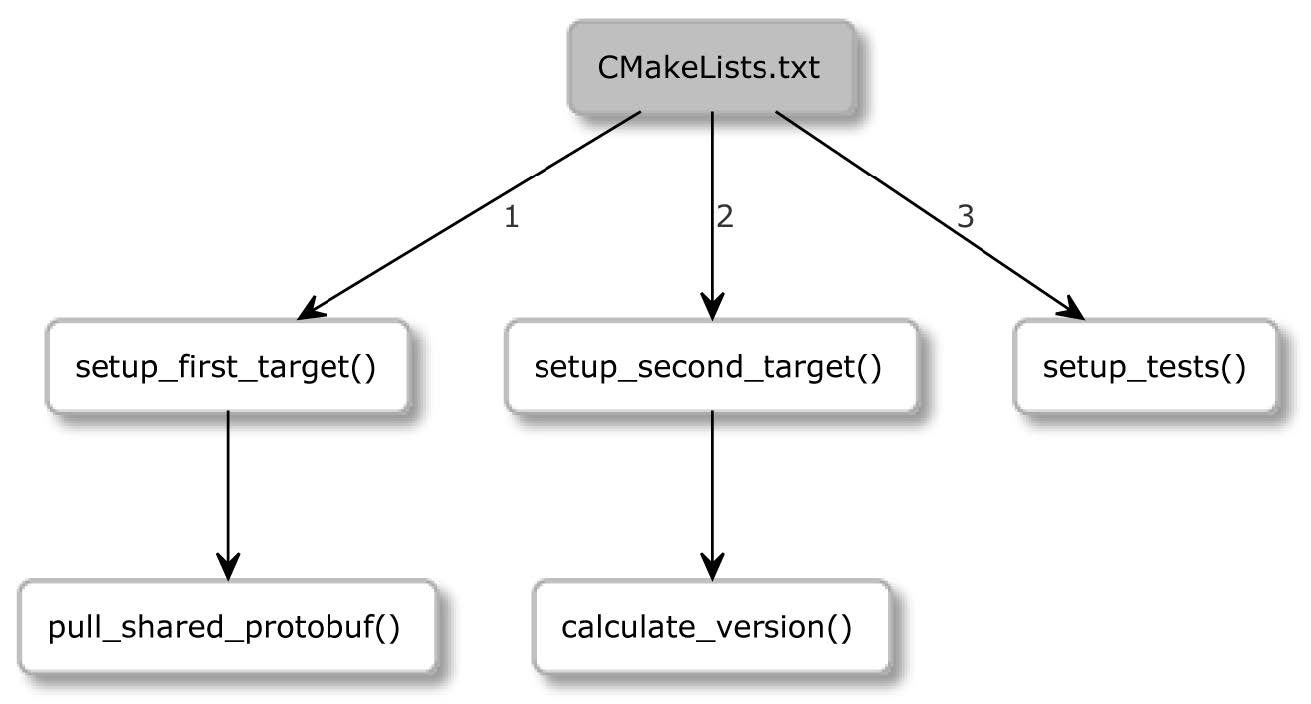
\includegraphics[width=0.8\textwidth]{content/1/chapter2/images/3.jpg}\\
Figure 2.3 – A procedural call graph
\end{center}

Writing in this procedural style is a bit of a problem in CMake – you are required to provide command definitions you're planning to use ahead of time. The CMake parser will not have it any other way. Your code would look something like this:

\begin{lstlisting}[style=styleCMake]
cmake_minimum_required(...)
project(Procedural)
function(pull_shared_protobuf)
function(setup_first_target)
function(calculate_version)
function(setup_second_target)
function(setup_tests)

setup_first_target()
setup_second_target()
setup_tests()
\end{lstlisting}

What a nightmare! Everything is reversed! This code is very difficult to read as the most minuscule details are at the top of the file. A correctly structured piece of code lists the most general steps in the first subroutine, after which it provides the slightly more detailed subroutines, and pushes the most detailed steps to the very end of the file.

There are solutions to this problem: moving command definitions to other files and partitioning scopes across directories (scoped directories will be explained in detail in Chapter 3, Setting Up Your First CMake Project). But there is also a solution that is simple and elegant: declaring an entry-point macro at the top of the file and calling it at the very end of the file:

\begin{lstlisting}[style=styleCMake]
macro(main)
function(...) # key steps
function(...) # details
function(...) # fine details
main()
\end{lstlisting}

With this approach, our code is written with gradually narrowing scope, and because we're not actually calling the main() macro until the very end, CMake won't complain about the execution of undefined commands!

One last question remains – why use a macro over a recommended function? In this case, it's good to have unrestricted access to global variables, and since we're not passing any arguments to main(), we don't need to worry about the usual caveats.

You'll find a simple example of this concept in the chapter-02/09-procedural/ CMakeLists.txt listfile in the GitHub repository for this book.

\hspace*{\fill} \\ %插入空行
\noindent
\textbf{A word on naming conventions}

Naming is famously hard in software development, but nevertheless, it's very important to maintain a solution that is easy to read and understand. When it comes to CMake scripts and projects, we should follow the rules of the clean code approach, as we would with any software development solution:

\begin{itemize}
\item 
Follow a consistent naming style (snake\_case is an accepted standard in the CMake community).

\item 
Use short but meaningful names (for example, avoid func(), f(), and suchlike).

\item 
Avoid puns and cleverness in your naming.

\item 
Use pronounceable, searchable names that don't require mental mapping.
\end{itemize}

Now that we know how to properly invoke the commands with the correct syntax, let's explore which commands will be the most beneficial to us to begin with.
















